\section{Problem Statement}\label{sec:problem_statement}

As shown in \cref{fig:gen_problem} this thesis will focus its attention on three critical challenges for FC EEG-based MI-BCI. First, despite the valuable insights derived from standard functional connectivity, it faces a performance deficit in MI classification tasks due to the inherently high noise in the EEG signals, issues of volume conduction, and notable inter-subject variability. Second, the heavy reliance on subject matter experts in FC-based feature extraction affects the system's efficiency. This dependence is amplified in scenarios where the same MI cognitive task generates various neural responses in different trials from the same subject, leading to poor and inconsistent predictions. Third, the importance of model transparency to achieve trust among users. With most of the complex models functioning as 'black boxes', predictions are made without clear justifications that can explain why certain decisions are chosen over others, which is crucial for understanding the cognitive processes occurring underneath.

\begin{figure}[!h]
    \centering
    \includegraphics[width=1.0\linewidth]{Figures/problem_statement/general_problem.pdf}
    \caption{Illustration of the three key challenges in FC EEG-based MI-BCI: noise and variability in single trial FC estimators, handcrafted-based subject-specific EEG-based MI-BCI Representation, and the need for model transparency}\label{fig:gen_problem}
\end{figure}


\subsection{Single-Trial FC MI Classification Inefficiency \label{sec:singlefc}}

While standard FC, extracted from various EEG recordings of the same cognitive process (multiple trials), provides invaluable insights for interpreting brain activity patterns, it often struggles to achieve high accuracy in MI classification tasks because single-trial FC estimation only gets a fraction of the data (one trial) \cite{chiarion2023connectivity, rodrigues2020single, billinger2013single}. Since FC quantifies the statistical dependencies between EEG channels, its accuracy estimation is heavily influenced by challenges such as a low signal-to-noise ratio, volume conduction problems, and inter-subject variability \cite{abiri2019comprehensive,bastos2016tutorial}. Therefore, single-trial estimation is an intricate task that usually yields MI classification inefficiency systems \cite{yang2021novel}. 

The inherent noise in signals recorded on the scalp significantly hinders the underlying neural activity, challenging the single-trial estimation from EEG data \cite{si2020predicting, hata2016functional}. Specifically, external or environmental artifacts such as electromagnetic interferences by lighting, AC power lines, and electronic devices; and noise arising from body activities like other cognitive processes, skin resistance fluctuations, electrocardiographic activity (heart functioning), electrooculographic activity (eye movements), electromyographic activity (any muscle movements), and respiration diminish the fidelity of EEG signals~\cite{nentwich2020functional, somers2018generic}. In addition, functional activities recorded using EEG show volume conduction problems even before they can be measured on the scalp's surface, causing several EEG channels to be correlated \cite{qiao2023eeg, varone2021machine}. As a result, many spurious connectivities are induced due to the low signal-to-noise ratio present in EEG signals, impeding competitive performance \cite{bakhshayesh2019detecting}.

Aside from these issues, individual brain activity's intrinsic diversity and complexity also lead to inter-subject variability \cite{wriessnegger2020inter}. The inter-subject variability is not considered a noise per se but an expression of the subjective motor process~\cite{saha2020intra}. For instance, single trial FC-based MI-BCI performance can be negatively affected by the fact that the motor learning process varies over subjects due to intrinsic human kinematic parameters, motivational components, and factors ranging from demographic variables like gender and age to psychological and physiological conditions such as fatigue, relaxation, concentration, and living habits \cite{antonakakis2020inter, huang2023discrepancy}. This is especially evident when different individuals imagine performing the same motor task, leading to varied SMR synchronization patterns that affect FC features~\cite{wriessnegger2020inter, xie2020review}.

Most of the existing single-trial FC estimation methods are based on covariance matrices calculated from the original EEG signal domain and do not account for brain activity's inherent nonlinearity and non-stationarity, inevitably compromising their accuracy \cite{cao2022brain, epmoghaddam2022epileptic, miladinovic2021effect}. Moreover, the high variance in brain activity during task execution adds further difficulties in identifying relevant feature patterns. While improvements in covariance matrix estimation might be achieved through mapping and regularization techniques, selecting an appropriate distance metric to encapsulate variability remains challenging \cite{wang2020diverse,congedo2017fixed}.

In summary, single-trial FC-based MI-BCI systems must enhance the model's accuracy without compromising its interpretability using innovative strategies to effectively manage the complex issues of nonlinearity, non-stationarity, and inter-subject variability. \cref{fig:problem_1} shows a representation of these challenges.

\begin{figure}[!h]
    \centering
    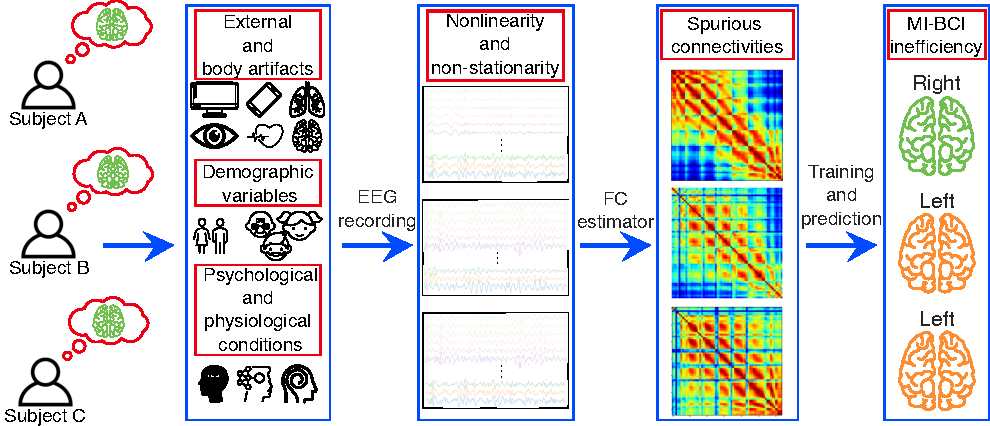
\includegraphics[width=1.0\linewidth]{Figures/problem_statement/problem1_FV.pdf}
    \caption{Single-trial FC-based MI classification inefficiency graphical scheme}\label{fig:problem_1}
\end{figure}


\subsection{Handcrafted-based Subject-Specific EEG-based MI-BCI Representation \label{sec:problem2}}

Despite the substantial progress made in the EEG signals representation in the MI-BCI field, functional connectivity analysis suffers from a high rate of spurious connections due to noise, affecting mainly the accuracy of low-performing individuals \cite{ismail2020graph,wang2020diverse,congedo2017fixed}. This noise within EEG signals significantly contributes to high variability, hindering the underlying neural activity and potentially leading to inaccurate interpretation \cite{caicedo2021deep}. Therefore, EEG signal representation still presents a significant challenge \cite{rashid2020current}.

These challenges arise predominantly from the complexity, degree of sensitivity, and necessity of human experts in EEG representation, such as artifact removal strategies and spatial, temporal, and frequency filtering \cite{chamola2020brain, padfield2019eeg} as graphically illustrated in \cref{fig:problem_2}. For instance, the handcrafted nature of EEG representation leads to high information loss and limits the capacity to detect discriminative correlations among EEG channels, particularly in low-performing individuals \cite{altaheri2023deep}.

While multiple strategies exist for addressing EEG representation issues that can be beneficial in facing MI classification inefficiency, they are often carried out by exhaustive search, limiting the range of artifact removal strategies and spatial, temporal, and spectral filtering selection that can be accomplished \cite{saha2020intra, ismail2020graph, meers2020motor, talukdar2019motor}. In addition, optimizing these steps proves particularly challenging when handling low-performing subjects, even with the insights from subject matter experts \cite{vidaurre2020sensorimotor}.

Despite the considerable advancements in the EEG signal representation within the MI-BCI field, the necessity for human expert intervention in the analysis still poses a significant challenge. In particular, formulating strategies for artifact removal and implementing spatial, temporal, and frequency filters can be exhaustively demanding, especially when dealing with low-performing subjects. The complexity and sensitivity of these strategies often result in a loss of crucial information and limitations in accurately identifying genuine connections between signals, even when guided by subject matter expert knowledge.

\begin{figure}[!h]
    \centering
    \includegraphics[width=1.0\linewidth]{Figures/problem_statement/problem2_VF.pdf}
    \caption{Illustration of challenges in EEG signal representation, including strategies for artifact removal and implementing spatial, temporal, and frequency filters \label{fig:problem_2}}
\end{figure}


\subsection{Lack of Transparency and Interpretability Strategies in MI-BCI \label{sec:problem3}}

The third significant challenge for FC-based MI-BCI systems is model transparency and interpretability, linking back to the core aim of Explainable AI (XAI), which seeks to provide meaningful insights into the reasoning behind model predictions, increasing the confiability, causality, transferability, accuracy, accessibility, and interaction \cite{smuha2019eu}. Integrating various features from different domains into MI-BCI systems poses a unique level of complexity \cite{guillot2019benefits}. For instance, complex models often act like ‘black boxes’, offering outcomes without explanations or justifications \cite{ras2018explanation}, as seen in \cref{fig:problem_3}.

Understanding why models favor specific predictions over others is crucial, not only for predictive efficiency but also in healthcare and medical decision-making scenarios \cite{miotto2018deep}. The interpretation process should highlight the prioritized features during model training and illustrate how these features' interrelationships impact such decisions \cite{zeiler2014visualizing, chakraborty2017interpretability}. As models become more refined, the need for transparency and interpretability amplifies, especially in clinical research where reliance on model recommendations is critical \cite{xiao2018opportunities}.

Moreover, the ongoing debate over the definition of interpretability leads to diverse interpretation methods \cite{fan2021interpretability}. Specifically for FC EEG-based MI-BCI, the challenge lies in creating a quantitative and qualitative interpretability framework that integrates the distinct contributions of each connection to classification across different MI tasks \cite{zuk2020eeg}. Identifying and excluding irrelevant features, especially those generated from noisy functional connectivity patterns, is crucial for model refinement, enhancing its generality, reducing overfitting risks, and expanding the use of MI-BCI in clinical applications like diagnosis, monitoring, and computer-assisted learning \cite{qian2018brain}.

In brief, one of the significant challenges in XAI within MI-BCI systems is ensuring model transparency and interoperability. However, introducing several features from different domains into these systems can be complex. This complexity is exacerbated by models that function like ‘black boxes,’ providing results without explanations. Understanding why specific predictions are favored and how interrelated features influence these decisions is crucial, especially in critical fields like healthcare. In the MI-BCI context, the task lies in forming a quantitative and qualitative framework that can map the individual contributions of each connection within different domains across varying MI tasks for optimizing the model, reducing overfitting risks, and expanding the clinical applications of MI-BCI.

\begin{figure}[!h]
    \centering
    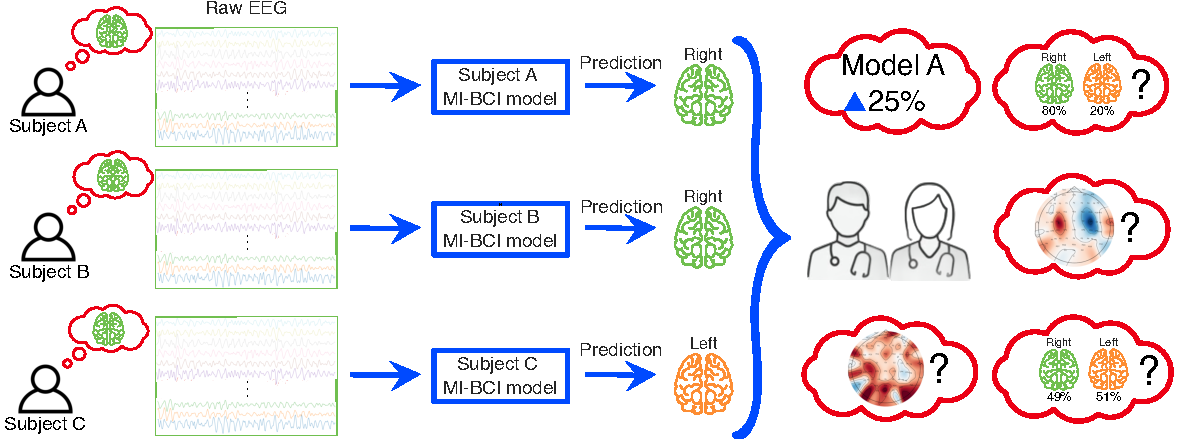
\includegraphics[width=1.0\linewidth]{Figures/problem_statement/problem3_FV.pdf}
    \caption{Transparency and interpretability challenges in MI-BCI models graphical scheme \label{fig:problem_3}}
\end{figure}


\subsection{Research Question}

Given the challenges identified in EEG-based MI-BCI systems, including single-trial FC inefficiency, complexities in EEG representation, and issues of transparency and interpretability in complex models, we propose the following research question:

How can a single-trail FC be developed to manage non-stationary EEG subject-specific representations, handle spurious connectivities, and encode non-linear spatial, temporal, and spectral discriminative and interpretable MI patterns?